\documentclass[10pt]{article}

\usepackage{tabularx}
\usepackage[a4paper,margin=2.5cm, bottom=2.5cm]{geometry}
\usepackage{fancyhdr}
\usepackage{listings}
\usepackage{booktabs}
\usepackage{float}
\usepackage{subcaption}
% \usepackage{caption}
% \captionsetup{font=footnotesize}
\usepackage{graphicx}
\usepackage{amsmath}
\usepackage{amssymb}
\usepackage{amsthm}
\usepackage{array}
\usepackage[table]{xcolor}
\usepackage{pgfplots}
\pgfplotsset{compat=1.17}
\usepackage{pgfplotstable}
\usepackage{multirow}
\usepackage{tikz}
\usepackage[hidelinks]{hyperref}
\usepackage{titling}
\usepackage[polish]{babel} % Polish language support

\setlength{\headheight}{40pt}
\setlength{\parindent}{0pt}
\setlength{\parskip}{1ex}
\renewcommand{\headrulewidth}{0pt}

\pagestyle{fancy}
\fancyhead{}
\fancyhead[L]{
    \renewcommand{\arraystretch}{1.5}
    \begin{tabularx}{\textwidth}{|X|X|}
        \hline
        \bfseries Obliczenia inteligentne & \bfseries \thetitle \\
        \hline
    \end{tabularx}
}
\fancyfoot[C]{\thepage}

\renewcommand{\maketitle}{
    \thispagestyle{plain}
    \renewcommand{\arraystretch}{2}
    \vspace*{-8em}
    \footnotesize
    \begin{flushleft}
        \begin{tabularx}{\textwidth}{|X|X|}
            \hline
            \bfseries Obliczenia Inteligentne  & \bfseries \thetitle                           \\ \hline
            \multicolumn{2}{|l|}{
                \begin{tabular}[t]{@{}ll@{}} 
                    \textbf{Grupa:} Grupa 1
                    \hspace{4.5em}
                    \textbf{Dzień i czas:} Czwartek, 10:00
                    \hspace{4.5em}
                    \textbf{Rok akademicki:} 2023/24
                \end{tabular}
            } \\ \hline
            \multicolumn{2}{|l|}{
                \begin{tabular}[t]{@{}l@{\hspace{10em}}l@{}} 
                    \textbf{Imię i nazwisko:} \textsc{Jakub Pawlak} & \textbf{Imię i nazwisko:} \textsc{Magdalena Paku\l a} 
                \end{tabular}
            } \\
            \hline
        \end{tabularx}
    \end{flushleft}
    \renewcommand{\arraystretch}{1}
}


\title{Projekt 2 --- Zadanie 2}

\captionsetup{font=small}

\newcommand{\plotAccuraciesFromLoggedMetrics}[1]{
    \begin{tikzpicture}
        \begin{axis}[
            width=\linewidth,
            height=.5\linewidth,
            legend pos = south east,
            grid = major,
            style = {font=\small}
        ]
            \addplot+[mark=none] table[x = epoch, y = train_acc] {#1};
            \addlegendentry{Training set accuracy};

            \addplot+[mark=none, orange] table[x = epoch, y = val_acc] {#1};
            \addlegendentry{Test set accuracy};
        \end{axis}
    \end{tikzpicture}
}


\begin{document}

\maketitle
\normalsize

\section{Eksperyment 1: Architektury sieci splotowej dla MNIST (Jakub Pawlak)}\label{sec:ex1-pawlak_mnist}

\subsection*{Pierwsza architektura}


\pgfplotstableread[col sep=comma]{data/kuba/mnist/large.csv}\kubaMnistLarge{}

\begin{figure}[H]\centering
    \begin{subfigure}[t]{.6\textwidth}
        \plotAccuraciesFromLoggedMetrics{\kubaMnistLarge}
        \caption{Wykres zmian accuracy}
    \end{subfigure}
    \hspace{2em}
    \begin{subfigure}[t]{.34\textwidth}
        \centering
        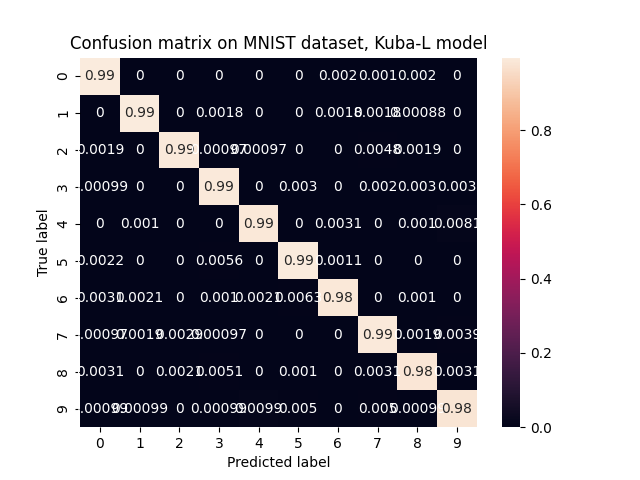
\includegraphics[width=\linewidth]{img/kuba/mnist/large_cm.png}
        \caption{Macierz pomyłek}
    \end{subfigure}
    \caption{Wyniki dla 1 architektury}
\end{figure}


\subsection*{Druga architektura, prowadząca do ekstrakcji 2 cech}

\pgfplotstableread[col sep=comma]{data/kuba/mnist/smol.csv}\kubaMnistSmol{}

\begin{figure}[H]\centering
    \begin{subfigure}[t]{.6\textwidth}
        \plotAccuraciesFromLoggedMetrics{\kubaMnistSmol}
        \caption{Wykres zmian accuracy}
    \end{subfigure}
    \hspace{2em}
    \begin{subfigure}[t]{.34\textwidth}
        \centering
        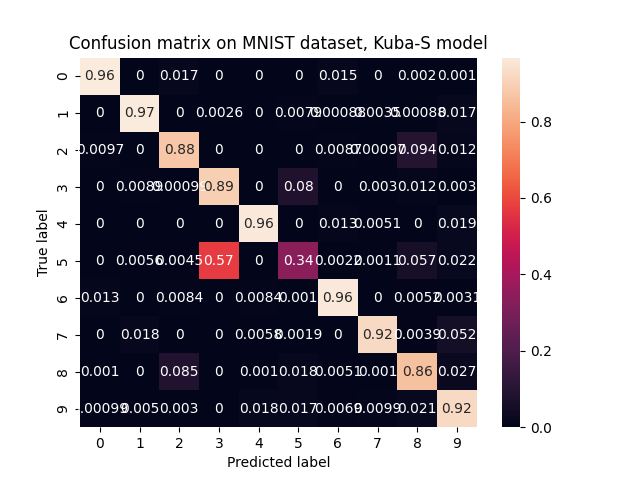
\includegraphics[width=\linewidth]{img/kuba/mnist/smol_cm.png}
        \caption{Macierz pomyłek}
    \end{subfigure}
    \caption{Wyniki dla 2 architektury}
\end{figure}

\pagebreak
\section{Eksperyment 1: Architektury sieci splotowej dla MNIST (Magdalena Pakuła)}\label{sec:ex1-pakula_mnist}

\paragraph{Pierwsza architektura}
\paragraph{Druga architektura prowadząca do ekstrakcji 2 cech}

\pagebreak
\section{Eksperyment 1: Architektury sieci splotowej dla CIFAR10 (Jakub Pawlak)}\label{sec:ex1-pawlak_cifar}

\paragraph{Pierwsza architektura}
\paragraph{Druga architektura prowadząca do ekstrakcji 2 cech}

\pagebreak
\section{Eksperyment 1: Architektury sieci splotowej dla CIFAR10 (Magdalena Pakuła)}\label{sec:ex1-pakula_cifar}

\paragraph{Pierwsza architektura}
\paragraph{Druga architektura prowadząca do ekstrakcji 2 cech}

\pagebreak
\section{Eksperyment 2: Wyniki dla MNIST}\label{sec:ex2_mnist}

\paragraph{Najlepsza architektura}
\paragraph{Najelpsza architektura prowadząca do ekstrakcji 2 cech}

\pagebreak
\section{Eksperyment 2: Wyniki dla CIFAR10}\label{sec:ex2_cifar}

\paragraph{Najlepsza architektura}
\paragraph{Najelpsza architektura prowadząca do ekstrakcji 2 cech}

\pagebreak
\section{Analiza i wnioski}\label{sec:wyniki}

\paragraph{Porównanie architektur sieci splotowych}

\paragraph{Wpływ augmentacji danych}

\end{document}